\section{Requirements}

\section{System Overview}
Table \ref{tab:pqmparameters} summarizes the 28 PQM parameters that has to be processed in the proposed system. To monitor this parameters, each PQM system has to have a sample rate of 20 kHz. To reduce data, every ten seconds the power line signal is captured for one second ($t_{n+1} - t_n = 10s$). Figure \ref{fig:sysdesign} shows this procedure. For visualization reasons, the plotted sine wave is not an actual snapshot of the power grid.

\begin{figure}[h]
	\centering
		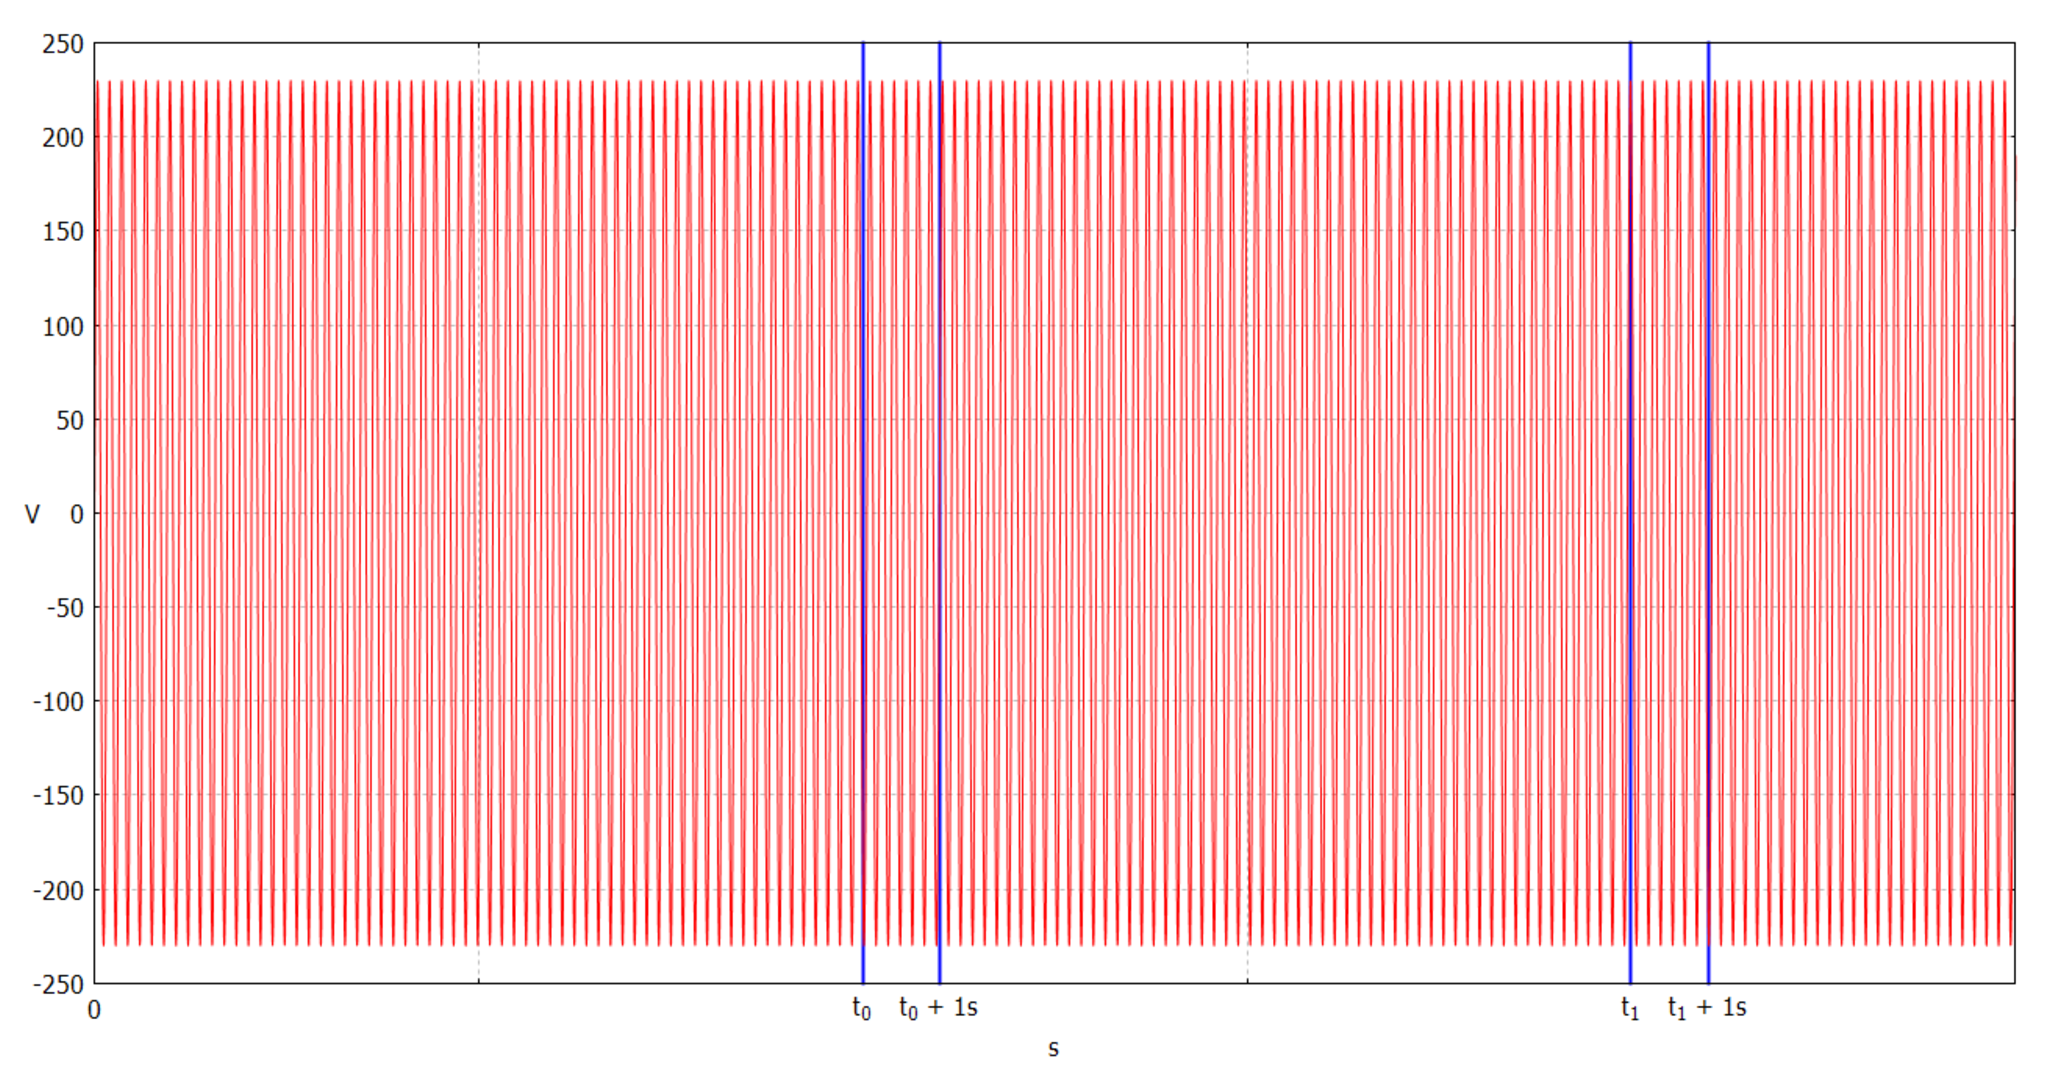
\includegraphics[scale=0.45]{graphics/sysdesign.eps}
	\caption{Signal capturing}
	\label{fig:sysdesign}
\end{figure}

According to this properties, three different types of data processing can be derived:

\begin{enumerate}
	\item Capture data on device, upload raw signal to the cloud for processing
	\item Capture data on device, process data on device, upload results to the cloud
	\item Option 2 with \textit{Dynamic Monitoring Frequency Scaling}
\end{enumerate}

Figure \ref{fig:BinDataPacket} show the binary representation of the data packets that are transferred from a PQM system to the cloud.

\begin{figure}[h]
	\centering
		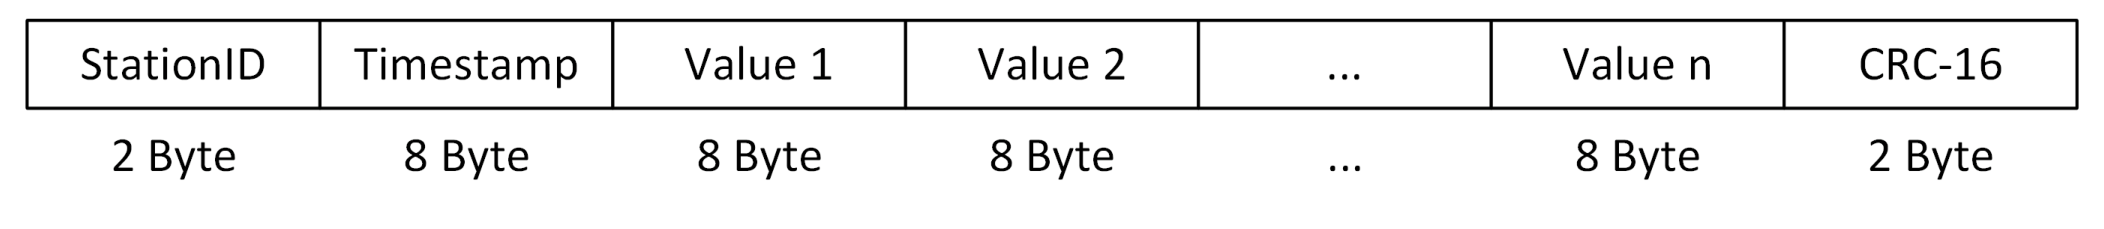
\includegraphics[scale=0.4]{graphics/BinDataPacket.eps}
	\caption{Binary data packet}
	\label{fig:BinDataPacket}
\end{figure}

When looking at the data packet, following assumptions can be derived for bandwidth and cloud-side storage:

\begin{enumerate}
	\item StationID + Timestamp + Signal + CRC-16 = 20 Bytes, 20 kHz sample rate \\ $\Rightarrow$ 390.625 kB/10s \textbf{$\Rightarrow$ 3.219 GB/d}
	\item Timestamp + 28 Values = 236 Bytes, 20 kHz sample rate \\ $\Rightarrow$ 236 B/10s \textbf{$\Rightarrow$ 1.94 MB/d}
	\item todo ...
\end{enumerate}

\section{Hardware Architecture}

\section{Software Architecture}

\subsection{Synchronization}
Synchronizing a distributed measurement system is essential. Although an not synchronized system delivers correct data that holds true for the point of measure, synchronizing theses systems allow to extract further knowledge out of the captured data. In the use case, selected for this thesis, power quality monitoring provides good arguments for synchronization. If somewhere in the power network an error occurs, it could be possible that this error is propagated throughout the network. Since the electric network and the infrastructure around it consists of resistive, inductive and capacitive load, a cascading of a fault is possible. With an adequate synchronization, it is possible to track the error propagation with a distributed measurement systems.

The testing equipment used in the proposed scenario support three different synchronization mechanisms. The radio based DCF77 time signal, the satellite based GPS signal and the Ethernet based SNTP protocol. The following section explains these three mechanisms in detail and evaluates which type suits most for this use case.

For the sake of completeness, two further synchronization modes exist. Distributed clock over EtherCAT and Q.sync. The first mode is part of the EtherCAT protocol that is implemented in the used modules, the second mode is a proprietary bus that connects multiple controllers. Since the different power quality measurement systems are spread across a wider geographical area, this two modes can't be used.

\subsubsection{DCF77}
DCF77 is a radio based time distribution services. It uses a long wave radio transmitter with a carrier frequency of 77.5 kHz. Due to the fact that the transmitter is located in Germany, it covers a maximum range (by using the proper detector) of approximately 2400 km, which is in fact whole Europe. Since DCF77 is driven by atomic clocks, the received radio signal is less accurate than the them\cite{dcf77}. Every minute, the time information (and additional information like civil warnings\cite{dcf77_2} and weather data\cite{dcf77}) is transmitted amplitude modulated (AM) and phase modulated (PM) in Binary Coded Decimal (BCD). In the current message the information about the next second is transmitted, furthermore, the start of a minute can be detected. It is possible to detect leap seconds and the switch to daylight-saving time \cite{dcf77_2}. Considering accuracy of the DCF77, the decoding mechanism is crucial. For the use in watches only the amplitude modulated signal is decoded which results in accuracy of +5ms up to +150ms. By using better antennas, this values can be enhanced to +5ms up to +15ms. To gain more accuracy, the phase modulated signal has to be decoded as well. This method results in an exactness of $\pm$2ms\cite{dcf77_3}.

Since the signal of a DCF77 receiver cannot be connected directly to the measurement devices, the signal has to be converter inside the receiver to a suitable format. As an example of such a format, the ''IRIG B003'' standard is described in more details here. The Inter Range Instrumentation Group (IRIG) specifies various standards regarding transmitting time information over via a serial time code format. The name of the described standard refers to a format with 100 pulses per second (B), Pulse width code (0), no carrier (0) and Binary Coded Decimal - BCD, Straight Binary Second of Day - SBS (3). The date information is transmitted as a sequence of seconds, minutes, hours, days, years, control functions and time of day \cite{irig}. Regarding the used testing equipment, DCF77 receivers can provide the IRIG B003 signal either straight as Transistor-Transistor Logic (TTL) signal into the measurement device or over the RS-485 bus.

\subsubsection{GPS}
The Navstar Global Positioning System (GPS) is a satellite based time distribution service. In normal operation mode, it consists of 24 geometrical space slots with at least one operational satellite in it. Each satellite sends it's time information, generated by an atomic clock, and it's position to the receiver stations down on earth with a frequency of 1.57542 GHz. To control and observer the status of the GPS, the Operational Control System (OCS) is used to communicate with the satellites via ground antennas. The OCS is responsible for various tasks including telemetry, monitoring of different parameters and uploading of navigation data. Considering accuracy, GPS offers two services. On the one hand, the Standard Positioning Service (SPS) that is available to the civil public with less accuracy and on the other hand, the Precise Positioning Service (PPS) available to the military of the USA and it allies with high accuracy.\cite{gps}. Due to this fact, the proposed system and the used testing equipment can only make use of the SPS.

% genauigkeit, receiver, augmentation system

After receiving the time information from one or more satellites, the data can be passed to the testing equipment. For this, the received information is transformed to the National Marine Electronics Association (NMEA) 0183 format. Since NMEA was designed as interconnection format of different devices used in the marine, the format consists of various sentences representing features of the connected devices. To use NMEA as protocol for transmitting time- and position data, the two sentences \$GPRMC (Recommended Minimum Navigation Information) and \$GPGGA (Global Positioning System Fix Data. Time, Position and fix related data for a GPS receiver) can be used. The data is transferred as ASCII text and can be decoded directly by knowing the format of the corresponding sentence. NMEA uses, like IRIG, a serial bus for communication\cite{nmea}.

Beside NMEA, some GPS receivers are also able to provide information via the previously described IRIG B003 format.

\subsubsection{SNTP}
The Simple Network Time Protocol (SNTP), as a subset of the Network Time Protocol (NTP), provides time information in a network to clients. If a client wants to synchronize it's internal clock with a clock placed in the network (SNTP server), it has to send a message to this server. In the response, three timestamps are transmitted. The client timestamp when the message was sent, server time when the message was sent and server time when the message was received. With the information in this message and the timestamp when this message was received by the client, the exact time can be applied to the client\cite{sntp}. To synchronize a client's clock, the offset and delay of the client relative to the server is computed. By the used algorithm (especially because of the 64 bit integer arithmetic) a client has to be at least 34 years in the past and at most 34 years in future in order to get synchronized by the SNTP server\cite{rfc5905}.

%genauigkeit

\subsubsection{Conclusion}
\todo{add some content here}

\section{Network Architecture}


\section{Security Aspects / Threat-Modeling}
\todo{check spelling}